\section{Introduction}
\label{sec:introduction}

% state the learning objective
\paragraph{} 
The objective of this laboratory assignment is to study and implement an AC/DC converter circuit while, at the same time, trying to maximize the figure of merit M. The AC/DC converter circuit is composed of two circuits: an Envelope Detector circuit, an electronic circuit that takes a (relatively) high-frequency amplitude modulated signal as input and provides an output, which is the demodulated envelope of the original signal, and a Voltage Regulator circuit, a system designed to automatically maintain a constant voltage.
The circuit can be seen in Figure~\ref{fig:circuit}.


\paragraph{}
In Section~\ref{sec:theoretical}, a theoretical introduction is made in order to contextualize all the main principles that sustain our analysis of the circuit. This circuit is carefully analysed in Section~\ref{sec:analysis}, where the results are obtained in GNU Octave. Also, in Section~\ref{sec:simulation}, the circuit is analysed by simulation through the use of NGSpice to simulate the electric circuit behaviour. The results of the simulation of Section~\ref{sec:simulation} are then compared to the theoretical results obtained in Section~\ref{sec:analysis} and the comparative results are expressed in Section~\ref{sec:erroranalysis}. The conclusions of this study are outlined in the final part of the report, in Section~\ref{sec:conclusion}.


\begin{figure}[h] \centering
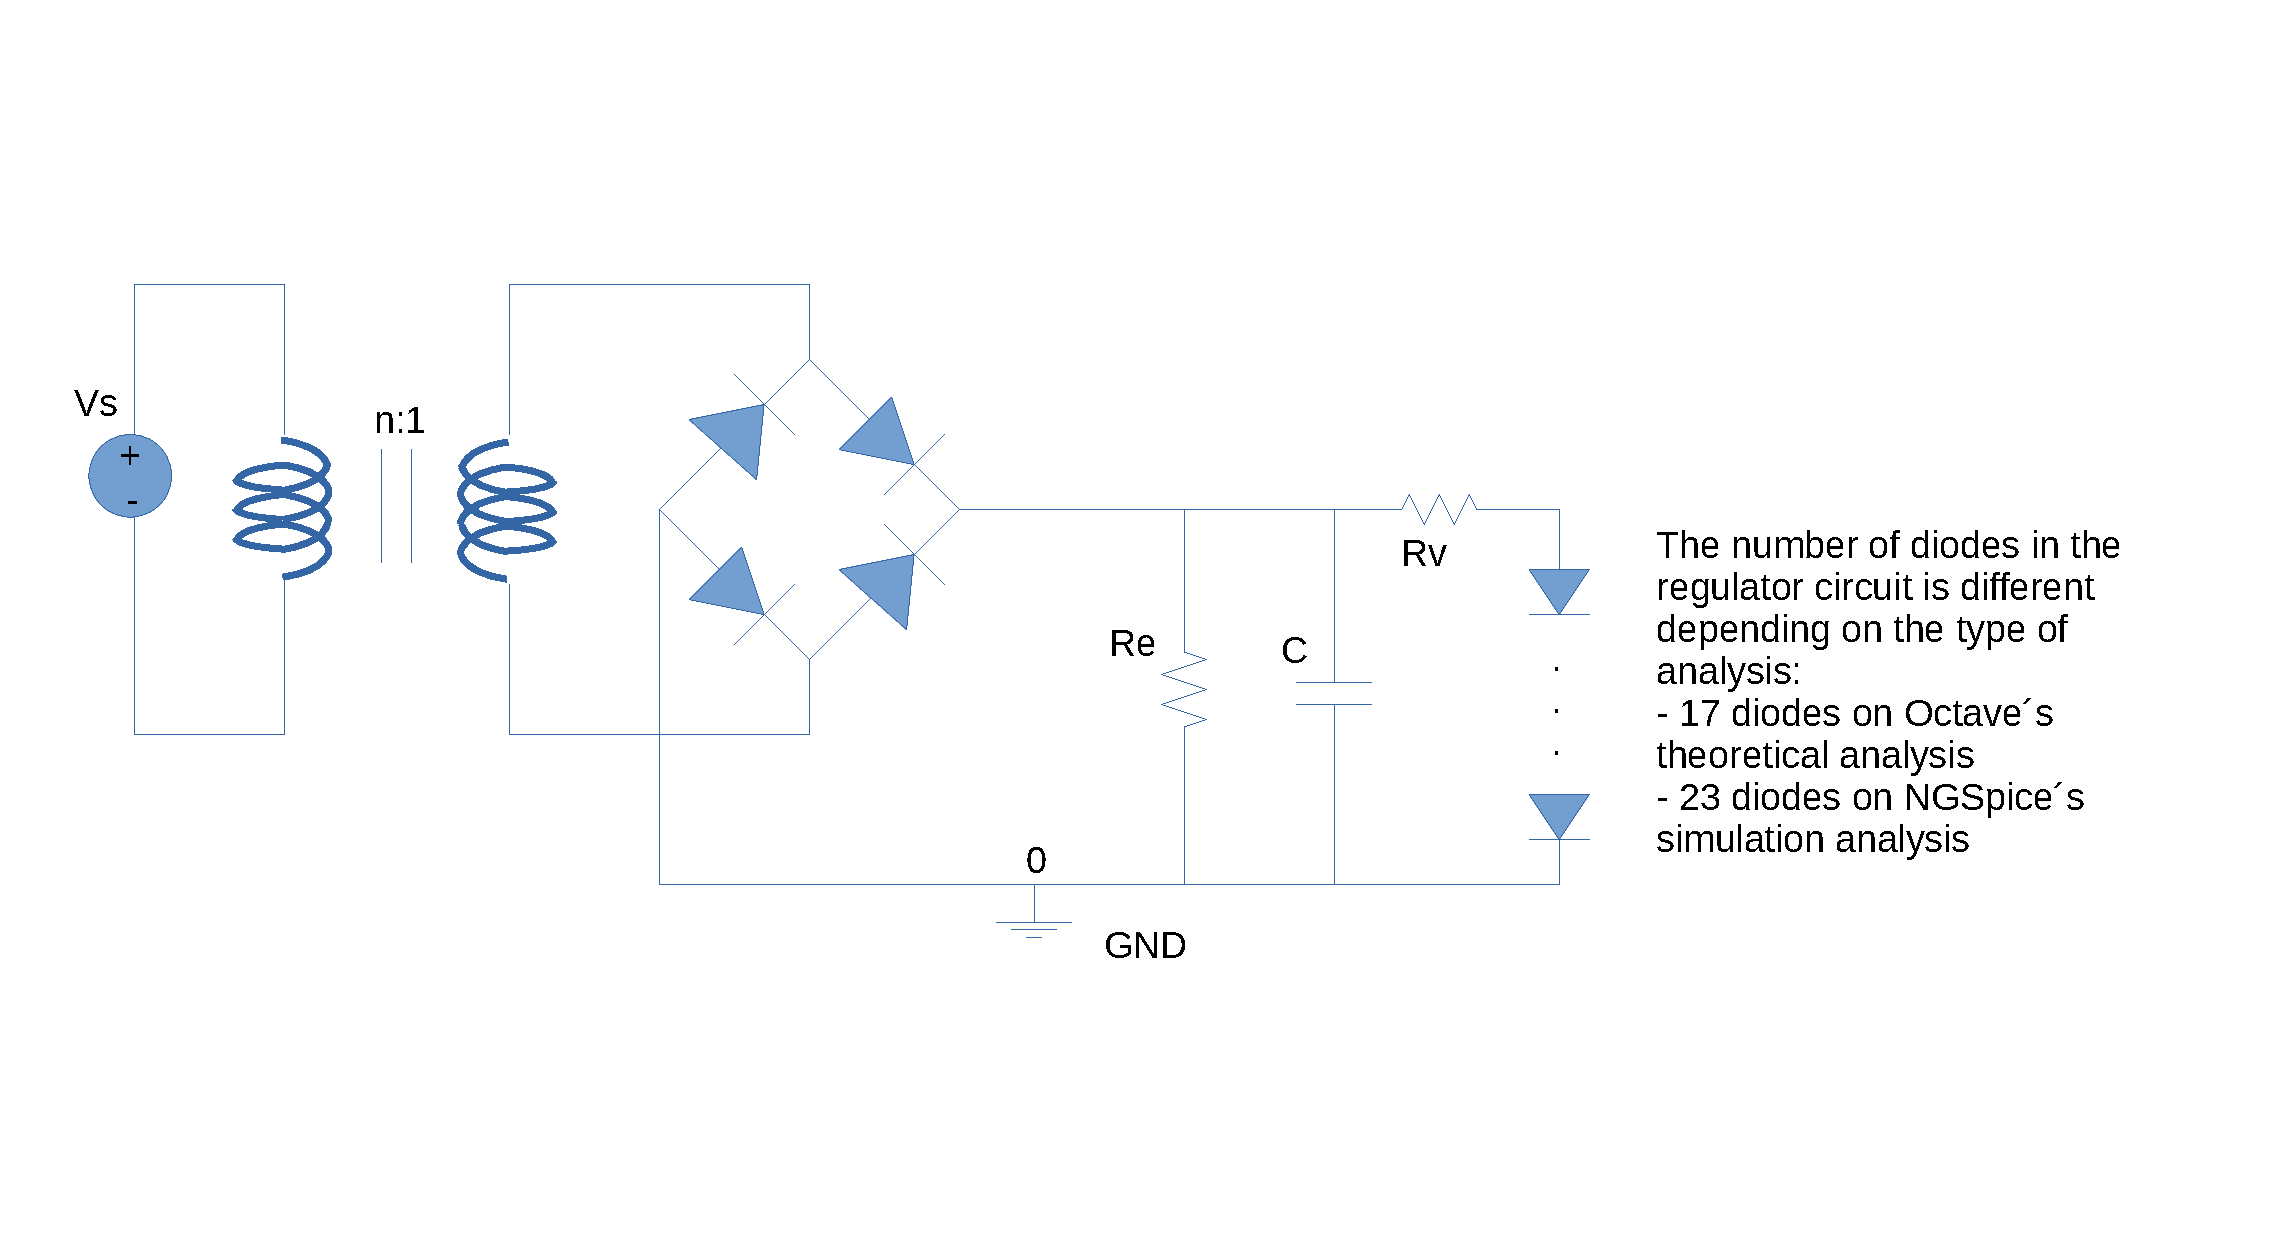
\includegraphics[width=0.4\linewidth]{circuit.pdf}
\caption{Third laboratory circuit.}
\label{fig:circuit}
\end{figure}

